
The following section will introduce the most important parts of the software for the project. The design of the software will be shown as a flow chart and described.
The section will focus on the feedback loop used, but will also go through some of the smaller parts, such as PWM and the code used for the CPLD.

Pulse Width Modulation is a very effective and straightforward way to control the speed of the robot rapidly. It works by limiting how long the of a given period the power is 'on' compared to 'off'.
PWM is used by utilizing Output Compare on the chip, which lets the chip generate pulses based on a timer. This is initialized in the following way:

\section{Software flowchart}
\img{figures/softwareflowchart.png}{Software flowchart}{softwareflowchart}{0.9}
\newpage
\section{Pulse-width modulation}
The robot utilizes pulse-width modulation by initiating a desired frequency, setting up the output compare, starting a timer, and then finally calculating the trigger timing of the timer.

\begin{lstlisting}
void initPWM() {
    int sysClk = 80000000; //FPB
    int pwmFreq = 1000; //Desired frequence
    int prescaleV = 1; 
    int dutyCycle = 0;
    
    PMCONbits.ON = 0; 
    PMAEN = 0;
    
    OC4CON = 0x0000; //Turn off the Output Compare while setting up
    OC4R = 0x00638000; //Config compare Register, rising edge
    OC4RS = 0x00638000; //Secondary compare Register, falling edge
    OC4CON = 0x0006; //Turn on Output Compare in PWM mode
    OC4RS = (PR4 + 1)*((float) dutyCycle / 100); //Sets the duty cycle, RS = time until falling edge starts
    OC4CONSET = 0x8020; //Enable peripheral,  bit 5: 0=16 bit compare mode, 1=32 bit
    
    OC5CON = 0x0000; //Same as above
    OC5R = 0x00638000;
    OC5RS = 0x00638000;
    OC5CON = 0x0006;
    OC5RS = (PR2 + 1)*((float) dutyCycle / 100);
    OC5CONSET = 0x8020;
    
    T2CONSET = 0x0008; //Starts a 32-bit timer
    T2CONSET = 0x8000; //Enables the timer

    PR4 = (sysClk / (pwmFreq * 2) * prescaleV) - 1; //Calculate how often the timer should trigger
    PR2 = (sysClk / (pwmFreq * 2) * prescaleV) - 1;
}
\end{lstlisting}
 
\subsection {Duty cycle}

The duty cycle is used to describe how long the power is 'on' compared to 'off'. A higher duty cycle will yield more energy than a low one. The software uses a frequency of 1000Hz, which makes it straightforward to calculate to real time, if this is needed - it also provides enough precision to make the motors responsive quickly.
The duty cycle can be changed by changing how long until the Output Compare sends a falling edge:

\begin{lstlisting}
void adjustDuty(int channel, int duty) {//The function takes an argument based on which motors PWM should change, and the desired duty cycle
    switch (channel) { 
        case 1:
            OC5RS = (PR2 + 1)*((float) duty / 100); //Sets the secondary register, to tell it how long until it should send a falling edge
            break;
        case 2:
            OC4RS = (PR4 + 1)*((float) duty / 100);
            break;
    }
}
\end{lstlisting}

\section{Feedback loop}
A feedback loop is a way of controlling how something, in this case a robot, behaves by receiving an output and adjusting the performance to match a desired output.\\
The robot made in this project utilizes a feedback loop by firstly turning towards a set goal, and then avoiding obstacles along the way through sensors measuring the distance from the robot to the obstacle. If an obstacle gets too close, the robot will turn away from the obstacle and head back towards the goal.
\subsection{Reading sensors}
To know how far away an object is, some form of sensor feedback is needed. In this case, 3 ultrasound sensors have been implemented. The microprocessor sends a turn-on signal to the sensors, starts a timer and then waits until the sensors return with their own signal. The time between the start and finish signal can then be used to calculate the distance between the robot and the object.\\
\begin{lstlisting}
long readUltrasonic(int channel){  
    long timerFinish = 0;
    long timerOld = 0;
    int timeout = 3000; //Sets a limit for how long the MCU waits for data
    switch(channel){ //Switches between the 3 sensors
        case 1:
            Trigger1 = 1; //Pin RG6
            DelayUs(10); //Sends a short pulse
            Trigger1 = 0;
            while(Echo1 == 0){} //Waits until pin RF6 is set to high
            timerOld = micros(); //Sets the start timer to time since the program started, in microseconds
            while(Echo1 == 1){ //While the sensors signal is high
                timerFinish = micros(); //Sets the end timer to check for timeout
                if(timerFinish - timerOld > timeout || timerFinish - timerOld < 0) //If the time to return is too high or below 0, return a default value
                    return 500;
            }
            break;
...
    }
    timerFinish = micros();
    long result = ((timerFinish-timerOld)*0.34)/2; //Calculate distance from speed of sound, divided by 2 since the sound wave also needs to return to the sensor.
    return result;  
}
\end{lstlisting}
The short pulse sent in the beginning of the function has been set by the manufacturer: \cite{HCSR04Datasheet}
\begin{figure}[!ht]
	\centering
	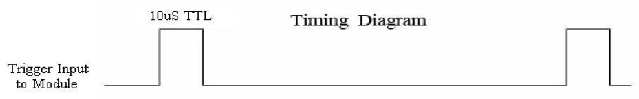
\includegraphics[width=0.7\textwidth]{figures/sensorTiming.PNG}
	\caption{\text{HC-SR04 timing diagram}}
	\label{Timing diagram}
\end{figure}

To reduce false sensor data, which there seems to be a lot of with these sensors, a rolling average has been implemented. This calculates the average of the previous 5 readings instead of a single reading, allowing the robot to ignore spikes in data.
\newpage
\subsection{Feedback}
The controller function takes the data from the 3 sensors and uses these to control how the robot should behave. The function is by no means fully optimized, but allows the robot to avoid obstacles in it's way.
\begin{lstlisting}
void controller(int midSensor, int rightSensor, int leftSensor){
    int midDistance = 100; //Sets the limit for the sensors, in millimetres
    int sideDistance = 50;
    if(midSensor < midDistance) //First check the middle sensor
    {
        brake(); //Stops the motors
        calculatePosition(); //Defunct, but should calculate where the robot is now in a coordinate system
        backwards(); //Starts backing away from the object
        int tachTarget = tach1-300; //Sets a tach target
        while(tach1 > tachTarget){} //Drives backwards until hitting the target
        brake(); //Brake again
        presetTurnLeft(); //Turn 30 degrees left
        brake();
        forwards(); //Start driving forwards again
    }
    else if(leftSensor < sideDistance)
    {
        int tachTarget = tach1-20; //Sets the target tach
        turnRight(); //Turn right
        while(tachTarget > tach1){} //Until target tach is hit
        brake(); //Brakes
    }
    else if(rightSensor < sideDistance) //Same as left, but reverse
    {
        int tachTarget = tach1+20;
        turnLeft();
        while(tachTarget < tach1){}
        brake();
    }
    else
        forwards(); //If no sensor is within the limit, just drive forwards
}
\end{lstlisting}
\newpage
\section{CPLD}
Compared to a regular microprocessor like the PIC32MX320F128H that is programmed in C converted to machine code in a procedural manner:
\begin{lstlisting}
if(this) {
	then this
} else {
	this
}
\end{lstlisting}
a CPLD is programmed with what is called Hardware description language or HDL for short.
instead of writing condition statements like you do in C, you define logic blocks and describe what that logic block do with the inputs and outputs given. \cite{HDL}
This allows for programming small logic circuits that act like several 74-series logic chips put together, but a CPLD can also be configured to contain a small microcontroller what internally can interpret machine code.\\ 
This make a CPLD a very powerful device since it can be configured to anything that can be made with pure logic circuitry, given that the selected CPLD have the needed amount of internal configurable logic blocks for the implementation. \cite{CPLD}
To simplify the programming, the IDE used to program the CPLD used on the motor shield, allows for programming by drawing schematics, which the IDE then synthensize and translate into the format the can be uploaded to the CPLD.\\
The CPLD on the motor shield is configured to allow full individual control of each h-bridge by using 4 control lines from the PIC32 to the CPLD for each h-bridge:
\begin{enumerate}
	\item[•]Enable
	\item[•]Direction A
	\item[•]Direction B
	\item[•]PWM
\end{enumerate}
Using these inputs without any logic control, allows for unwanted configurations of the h-bridge that will cause the power supply to be shortet to ground, this issues have been solved by programming the CPLD with a logic block that does not allow the configuration to occur, no matter the configuration of the input to the CPLD.\\
\ref{hbridgecpldlogic} shows the logic configurations of one of the two logic blocks that have been programmed into the CPLD.

\begin{figure}[!ht]
	\centering
	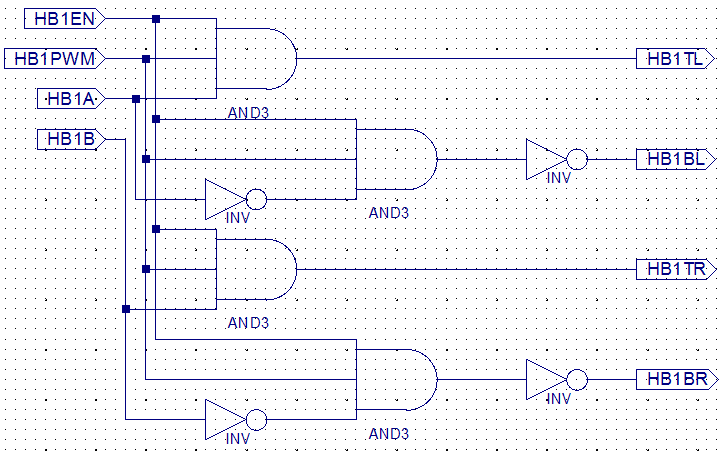
\includegraphics[width=0.8\textwidth]{figures/cpldlogic.png}
	\caption{\text{Single h-bridge logic block}}
	\label{hbridgecpldlogic}
\end{figure}
\newpage
%\img{figures/cpldlogic.png}{Single h-bridge logic block}{hbridgecpldlogic}{0.8}

\section{Part conclusion}
A few issues occurred during the development of the software,
\fixme{Software problemer og løsninger}
Another consideration has been to implement a real time system, such as RTOS, for the program. RTOS would make it possible for the sensors to be read simultaneously instead of one after the other. This could make a huge difference in time constricted systems, however, the system used in this project does fine without, since reading all 3 sensors take less than 10 ms.\\

Due to time constraints, a few requirements for the project have not been met. These include the need for line following capabilities, localization and the ability to return to a path that leads to goal.